\hypertarget{shapefunction_8h}{
\section{src/shapefunction.h File Reference}
\label{shapefunction_8h}\index{src/shapefunction.h@{src/shapefunction.h}}
}
Function for interpolation of basic variables. 

{\tt \#include \char`\"{}LMX/lmx.h\char`\"{}}\par


Include dependency graph for shapefunction.h:\nopagebreak
\begin{figure}[H]
\begin{center}
\leavevmode
\includegraphics[width=75pt]{shapefunction_8h__incl}
\end{center}
\end{figure}


This graph shows which files directly or indirectly include this file:\nopagebreak
\begin{figure}[H]
\begin{center}
\leavevmode
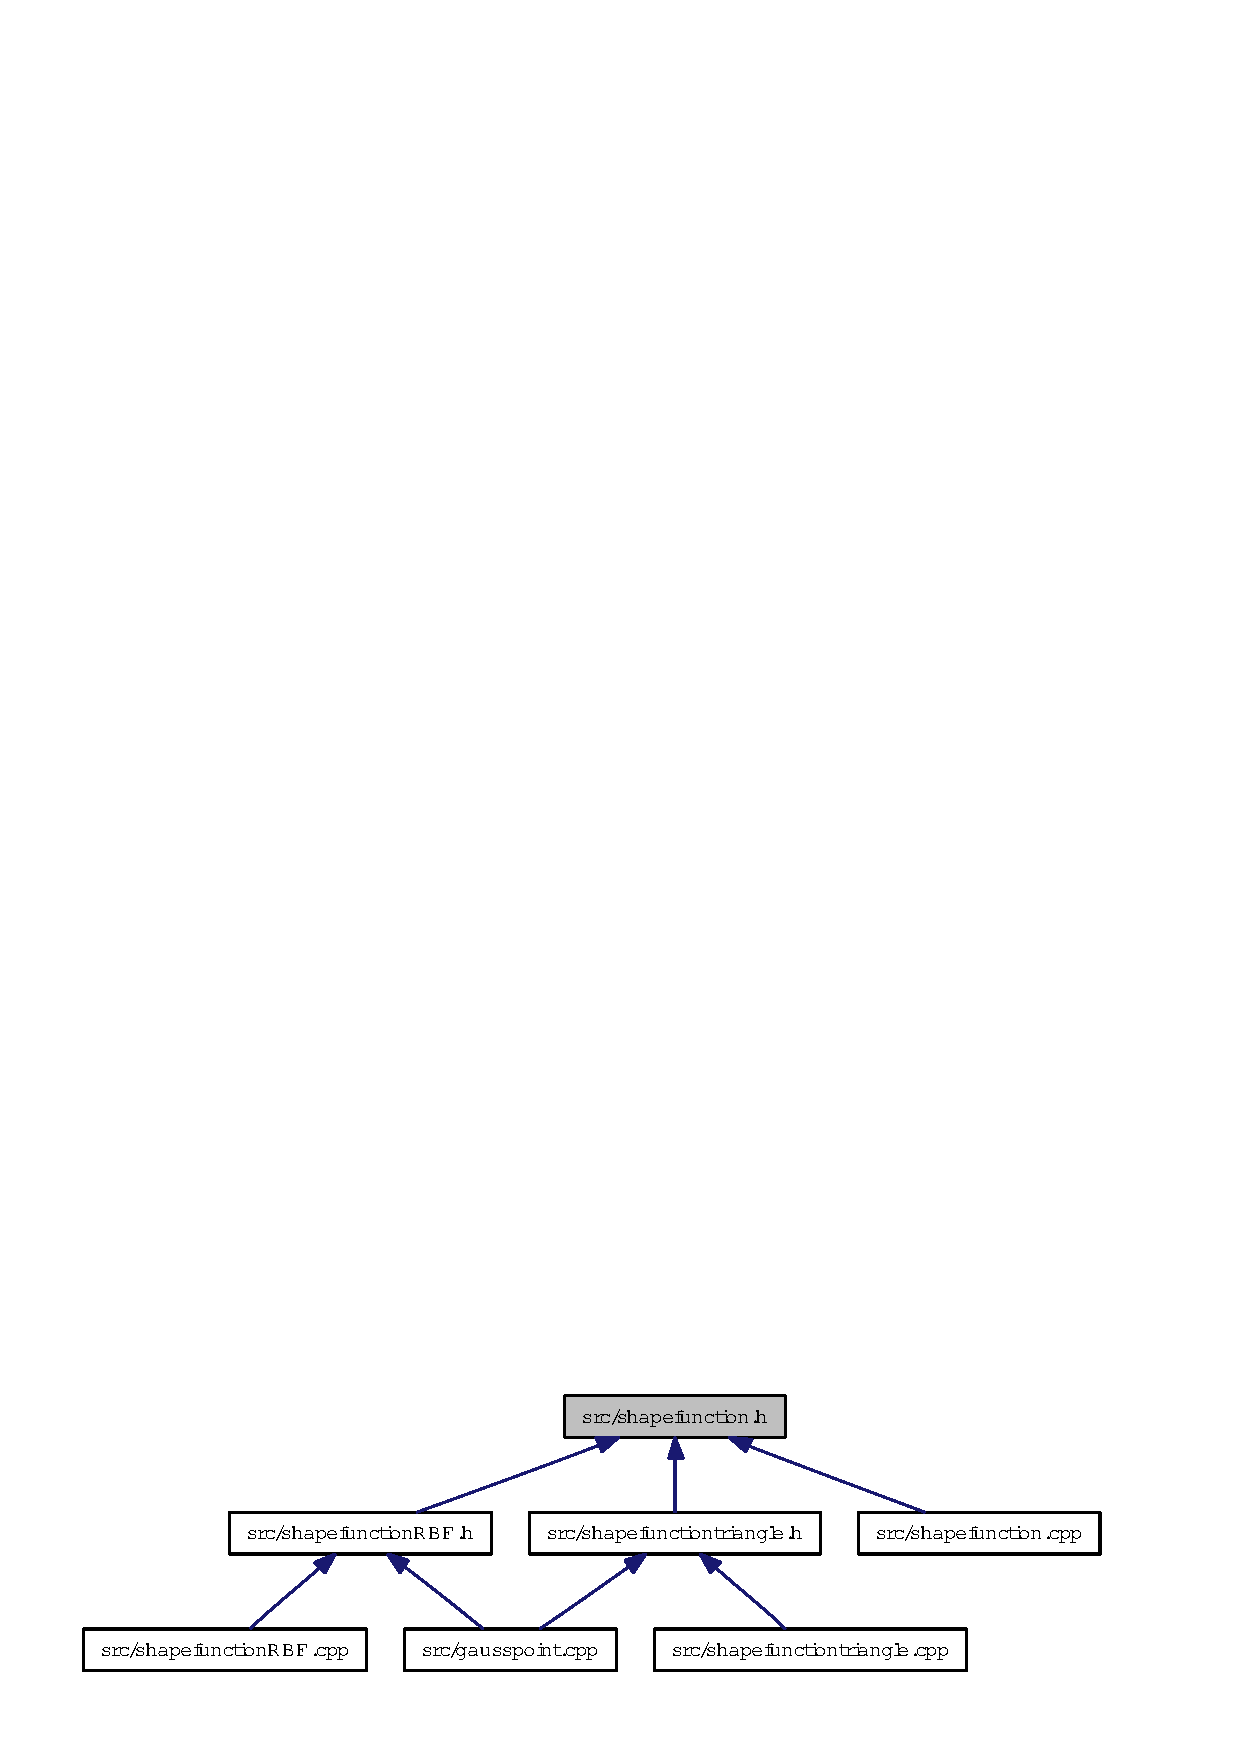
\includegraphics[width=266pt]{shapefunction_8h__dep__incl}
\end{center}
\end{figure}
\subsection*{Namespaces}
\begin{CompactItemize}
\item 
namespace \hyperlink{namespacemknix}{mknix}
\end{CompactItemize}
\subsection*{Classes}
\begin{CompactItemize}
\item 
class \hyperlink{classmknix_1_1ShapeFunction}{mknix::ShapeFunction}
\end{CompactItemize}


\subsection{Detailed Description}
Function for interpolation of basic variables. 

\begin{Desc}
\item[Author:]Daniel Iglesias Ibáñez \end{Desc}


Definition in file \hyperlink{shapefunction_8h-source}{shapefunction.h}.